
\chapter{Kramer Rate Theory}\label{kramer}
\lhead[\fancyplain{}{\bfseries\thepage}]{\fancyplain{}{\bfseries\rightmark}}
In this Chapter we make a briefly introduction in stochastic process and in Kramer Rate Theory.
\section{Fokker-Planck equation}
Fokker-Planck equation is a second order parabolic partial differential equation, and it's born during the investigation of the Brownian motion in a radiation field by Fokker and Planck \cite{K50}. This equation describe the time evolution of a probability distribution $\rho(x,t)$ in a stochastic process.
In one dimension, the Fokker-Planck equation (FPE) takes the simple form:
\begin{equation}
\frac{\partial \rho(x,t)}{\partial t} = -\frac{\partial}{\partial x} \biggl(A(x,t) \rho(x,t)\biggr) + \frac{1}{2} \frac{\partial ^2}{\partial x^2} \biggl(B(x,t) \rho(x,t) \biggr)
\label{eq:FP}
\end{equation}
with the initial condition:
\begin{equation}
\rho(x,t_0|x_0,t_0) = \delta(x-x_0)
\end{equation}
The first term in the equation ~\ref{eq:FP} is the drift equation, while the last term is the diffusion equation.
Every stochastic process described by a conditional probability satisfying the FPE is equavalent to the Ito stochastic differential equation (SDE)
\begin{equation}
dx(t) = A(x(t),t)dt + \sqrt{B(x(t),t)} dw_t
\end{equation}
and the two descriptions are complementary to each other.


\section{Bistability and Escape Problems}
In Nature exist some systems which have at least two possible stable states. This kind of systems are known as \emph{bistable systems} \cite{K50}. For such systems there are some problems of interest:
\begin{itemize}
\item How stable are the various states relative to each other?
\item How long does it take for a system to switch spontaneously from one state to onother?
\item How is the path in the relevant state space?
\item How does a system relax from an unstable state?
\end{itemize}
These questions can all be answered reasily for one-dimensional diffusion processes.
\subsection{Diffusion in a Double-Well Potential in one dimension}
We consider the system in which we have the probability density $\rho(x,t)$ of a prarticle, which obeys the Fokker-Planck equation:
\begin{equation}
\frac{\partial \rho}{\partial t } = \frac{\partial}{\partial x} U'(x)\rho + D \frac{\partial ^2 }{\partial x^2} \rho
\end{equation}
The shape of $U(x)$ is shown in Figure \ref{fig:kr}.
\begin{figure}[h]
\centering
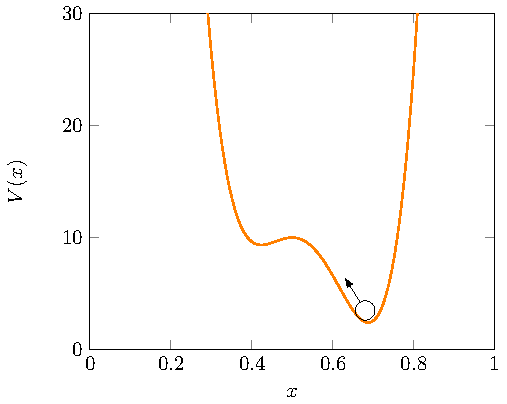
\includegraphics[scale=1.2]{images/kramerwell.pdf}
\caption{\emph{Example of double-well potential.}}
\label{fig:kr}
\end{figure}

There are two minima at $a$ and $c$ and in between, a local maximum $b$. The stationary distribution is
\begin{equation}
\rho_s(x) = \mathcal{N} e^{-\frac{U(x)}{D}}
\end{equation}
where $\mathcal{N}$ is the normalization constant.This distribution explains the bistability of the system, since, we have two local maxima of the potential in $a$ and $c$. (see Figure \ref{fig:kramerpot}).

\begin{figure}[h]
\centering
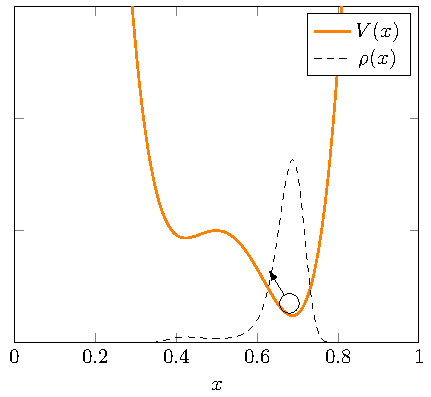
\includegraphics[scale=1.2]{images/kramerpot.pdf}
\caption{\emph{The distribution (dashed) explains the bistability of the system, since, we have two local maxima of the potential in $a$ and $c$..}}
\label{fig:kramerpot}
\end{figure}

\subsection{Behaviour for $D=0$}
In this case, $x(t)$ obeys the differential equation
\begin{equation}
\frac{dx}{dt} = - U'(x)
\end{equation}
with initial condition $x(0) = x_0$.
Now, since
$$
\frac{dU(x)}{dt} = U'(x)\frac{dx}{dt} = - (u'(x))^2 < 0 
$$

$x(t)$ always moves in such a way as to minimise $U(x)$, and stops only when $U'(x)$ is zero. Thus, depending on whether $x_0$ is grater than or less than $b$, the particle ends up at $c$ or $a$, respectively. Once the particle is at $a$ or $c$, it stays there. If it starts exactly at $b$, it also stay there, thoug the slightest perturbation drives it to $a$ or $c$. Thus, $b$ in an \emph{unstable} stationart point and $a$ and $c$ are stable.
\subsection{Behaviour if $D$ is small}
With the addition of noise, the situation changes. The stationary state can be approximated asymptotically as folows. Assuming $U(x)$ is everywhere sufficiently smooth, we can write
\begin{equation}
\begin{split}
U(x) & \simeq U(a) + \frac{1}{2} U''(a)(x-a)^2 \\
& \simeq U(c) + \frac{1}{2} U''(c)(x-c)^2 
\end{split}
\end{equation}
for $|x-a|$ and $|x-c|$ small, respectively.
If $D$ is very small, then we may approximate
\begin{equation}
\begin{split}
\rho_s(x)  &\simeq \mathcal{N} \exp\biggl(-\frac{U(a)}{D} - \frac{1}{2} U''(a)\frac{(x-a)^2}{D}\biggr) \\
&\simeq \mathcal{N} \exp\biggl(-\frac{U(c)}{D} - \frac{1}{2} U''(c)\frac{(x-c)^2}{D}\biggr) 
\end{split}
\label{eq:r}
\end{equation}
And zero elsewhere.
So that:
\begin{equation}
\mathcal{N}^{-1}  \simeq e^{-\frac{U(a)}{D}} \sqrt{\frac{ 2 \pi D }{U''(a)}} + e^{-\frac{U(c)}{D}} \sqrt{\frac{ 2 \pi D }{U''(c)}}
\end{equation}
Now suppose as in drawn in Figure \ref{fig:kramerpot} 
$$
U(a)>U(c)
$$
Then for small enough $D$, the second term is larger than the first and $\mathcal{N}^{-1}$ can be approximated by it alone. So, substituing into ~\ref{eq:r} we find
\begin{equation}
\rho_s(x) = \sqrt{\frac{U''(c)}{2 \pi D}} \exp\biggl(-\frac{1}{2}U''(c)\frac{(x-c)^2}{D}\biggr)
\end{equation}
for 
$$
|x-c| \sim \sqrt{D}
$$
and zero otherwise.
This means that in the limit of very small $D$, the deterministic stationary state at which $U(x)$ has an absolute minimum is the more stable state in the sense that in the stochastic stationary state, $\rho_s(x)$ is very small everywhere except in its immediate vicinity. This means, differently from the previous results, that due to the noise the  equilibrium points $a$ and $c$ are no longer equally stable.














\section{Kramer Rate Theory}
We consider the Smoluchowski equation:
\begin{equation}
dx = -V'(x)dt + \sqrt{2T} dw_t
\end{equation}

\begin{figure}
\centering
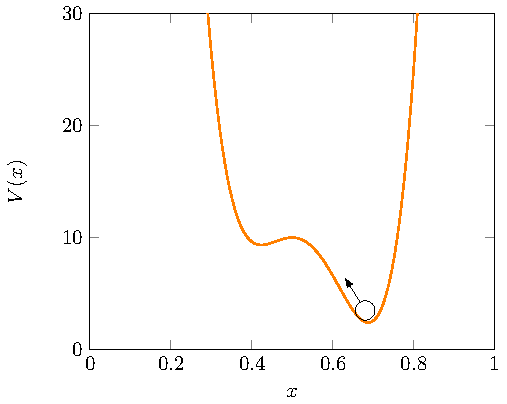
\includegraphics[scale=1.2]{images/kramerwell.pdf}
\caption{\emph{Example of double-well potential.}}
\label{fig:kr}
\end{figure}


where $V(x)$ is a double well potential with $x_a$ and $x_c$ local minima separated by a saddle point $x_b$: To compute the transition probability from the left well to the right well we consider the stationary solution of the Fokker-Planck equation:
\begin{equation}
\frac{\partial \rho}{\partial t } = \frac{\partial}{\partial x} U'(x)\rho + T \frac{\partial ^2 }{\partial x^2} \rho
\end{equation}

with the boundary condition that we have a source in the point $x_{-} < x_a$ and an absorbing boundary at the point $x_{+} > x_c$. We assume that the temperature $T$ is much les of the potential barrier $V_b - V_a$ and we look for a solution that reduces to the form:
$$
e^{-\frac{V(x)}{T}}
$$
in the vicinity of the point $x_a$ that vanishes at the absorbing barrier and gives a constant current $J$ between the two wells. Let
\begin{equation}
\rho(x)=C(x)e^{-\frac{V(x)}{T}}
\end{equation}
and the particle density current $-J=V'(x)\rho + \frac{\partial \rho}{\partial x}T$ reads
$$
V'(x)C(x)e^{-\frac{V}{T}} + C'(x)Te^{-\frac{V}{T}} - V'(x)C(x)e^{-\frac{V}{T}} = -J
$$
so that: 
$$
C'(x) = -\frac{J}{T}e^{\frac{V}{T}}
$$
and we integrate with the condition $C(x_{+}) = 0$:
$$
C(x) = \frac{J}{T}\int_{x}^{x_{+}} e^{\frac{V(y)}{T}}dy
$$

The distribution reads:
$$
\
ho(x) = \frac{J}{T} e^{-\frac{V(x)}{T}}\int_x^{x_{+}}e^{\frac{V(y)}{T}}dy.
$$

When$x \simeq x_a$ the integral
$$
\int_x^{x_{+}}e^{\frac{V(y)}{T}}dy
$$
is stationary since $V^(x_a) = 0$ and $\
ho(x)$ has the behavior of $e^{-\frac{V(x)}{T}}$.
Then we have to compute the number of particles $n_a$ in the left well
$$
n_a = \frac{J}{T}\int_{-\infty}^{x_{b}} e^{-\frac{V(x)}{T}} \int_{x}^{x_+} e^{\frac{V(y)}{T}} dy dx
$$

We approximate the integrals using the saddle point method:
$$
e^{\frac{V(y)}{T}} \simeq e^{\frac{V_b}{T} - \frac{\omega^2_b}{2T}(y-x_b)^2}
$$
$$
e^{\frac{V(x)}{T}} \simeq e^{\frac{V_a}{T} - \frac{\omega^2_a}{2T}(x-x_a)^2}
$$

so we compute:
$$
\frac{n_a}{J} = \frac{1}{T} e^{\frac{V_b-V_a}{T}}\int_{-\infty}^{x_b}dxe^{-\frac{\omega_a^2}{2T}(x-x_a)^2}\int_x^{x_+}e^{-\frac{\omega_b^2}{2T}(y-x_b)^2 }dy
$$
Then we can extend both the integrals between $-\infty$ and $+\\infty$:
$$
\int_{-\infty}^{+\infty}dxe^{-\frac{\omega_a^2}{2}(x-x_a)^2} = \frac{\sqrt{2 \pi T}}{\omega_a}\frac{n_a}{J}=\frac{2\pi}{\omega_a\omega_b}e^{\frac{V_b-V_a}{T}}
$$
And we find the transition probability rate:
$$
k_{a\to c} = \frac{J}{n_a} \simeq \frac{\omega_a \omega_b}{2 \pi} e^{\frac{V_b-V_a}{T}}
$$

\section{First passage time and transition rate escaping from a barrier}
We first consider the generic diffusion problem 
$$
\frac{\partial \rho}{\partial t} (x,t) = \mathbb{L}_{FP} \rho(x,t)
$$
where $\mathbb{L}_{FP}$ is a generic Fokker-Planck operator and we assume that $x \in \Omega$ and $\partial \Omega$ is an absorbing boundary condition: $\rho(x,t) =0 $ for $x\in \partial \Omega$ $\forall t$. By definition the probability to be in $\Omega$ at time $t$ for an initial condition $\delta(x-a)$ is:
$$
P_{\Omega} = \int_{\Omega} \rho(x,t|a)dx 
$$

Let $t_a$ the first passage time at $\partial \Omega$ for a realiation starting from $a$ at $t=0$ and let $p(t|a)$ be the probability distribution, we have by definition 
$$
\int_t^{\infty} p(s|a)ds = P_\Omega(t|a)
$$
since $\partial \Omega$ is an absorbing boundary condition. Then
$$
p(t|a) = \int_{\Omega} \frac{\partial}{\partial t} \rho (x,t|a)dx = \int_{\Omega} \mathbb{L}_{FP} \rho(x,t|a)dx
$$
To get an equation for the average first passage time $\tau(a)$
$$
\tau(a) = \int_{0}^{\infty} t p(t|a) dt = \int_{\Omega}\int_{0}^{\infty} t \frac{\partial}{\partial t} \rho(x,t|a)dt dx = - \int_{0}^{\infty} \int_\Omega \rho(x,t|a)dx dt
$$

we use the adjoint operator $\mathbb{L}_{FP}^{\dagger}$ and taking into account the boundary conditions 
$$
\mathbb{L}_{FP}^{\dagger} \tau(a) = -\int_{0}^{\infty}\int_{\Omega} \mathbb{L}_{FP}^{\dagger} \rho(x,t|a)dx dt
$$
Remark: $\mathbb{L}_{FP}^{\dagger}$ acts on the initial state $a$. From the Kolmogorov relation for Markov processes we get 
$$
\frac{\partial}{\partial s} \int_{\Omega} dt \rho(x,t|x_0,s)\rho(x_0,s|a,0)dx_0 = 0
$$

so that 
\begin{equation}
\begin{split}
& \int_{\Omega} dx_0 \rho(x_0,s|a,0)\frac{\partial}{\partial s} \rho(x,t|x_0,s) + 
\rho(x,t|x_0,s) \frac{\partial}{\partial s} \rho(x_0,s|a,0)
  = \\ 
& \int_{\Omega} dx_0 \rho(x_0,s|a,0)  \frac{\partial}{\partial s} \rho(x,t|x_0,s) + 
 \rho(x,t|x_0,s) \mathbb{L}_{FP} \rho(x_0,s|a,0)
\end{split}
\end{equation}
Then:
$$
\int_{\Omega} dx_0 \biggl[ \frac{\partial}{\partial s} \rho(x,t|x_0,s) + \mathbb{L}_{FP}^{\dagger} \rho (x,t|x_0,s) \biggr] \rho(x_0,s|a,0) 
$$
and since we consider a stationary process 
$$
\frac{\partial}{\partial s} \rho(x,t|x_0,s) = \frac{\partial}{\partial s} \rho (x,t -s|x_0,0) = - \frac{\partial}{\partial t} \rho(x,t-s|x_0,0)
$$
Letting $s \to 0$, one gets the adjoint equation
$$
\frac{\partial}{\partial t } \rho(x,t|a,0) = - \mathbb{L}_{FP}^{\dagger} \rho(x,t|a,0)
$$

Accoring to the previous result, the average first passage time reads
$$
\mathbb{L}_{FP}^{\dagger} \tau(a) = - \int_{0}^{\infty} \int_{\Omega} \mathbb{L}_{FP}^{\dagger} \rho(x,t|a)dx dt = \int_{\Omega}\int_{0}^{\infty} \frac{\partial}{\partial t} \rho(x,t|a,0)dt dx = - \int _{\Omega} \delta (x-a ) dx = -1
$$
 since $\lim_{t \to \infty} \rho(x,t|a) = 0 $ due to the presence of the absorbing boundary condition.
In an explicit form we have the equation 

\begin{equation}
\mathbb{L}_{FP}^{\dagger} \tau(a) = -1
\end{equation}

We remark that the computation of the average first passage time requires the knowloedge of the evolution at all times, however this result can be related to the escape probability rate. Let us apply the first passage time to the computation of the Kramer probability escape from a potential well.
We start from the Fokker-Planck equation 
$$
\frac{\partial}{\partial x} \frac{\partial V}{\partial x} \rho + D \frac{\partial ^2 \
\rho }{\partial x^2} = \frac{\partial 
\rho }{ \partial t}
$$
where the potential $V(x)$ has a minimum at $x = x_0$ and a saddle point at $x = x_1$.
The average firste time $\tau(x)$ id written:
$$
-\frac{\partial V}{\partial x}\frac{\partial \tau}{\partial x} + D \frac{\partial ^2 \tau}{\partial x^2} = -1
$$
and we get 
$$
\frac{\partial}{\partial x} \exp \biggl(-\frac{V(x)}{D}\biggr) \frac{\partial \tau}{\partial x} = - \frac{1}{D} \exp \biggl( - \frac{v(x)}{D}\biggr)
$$

The previous equation can be integrated
$$
\frac{d\tau}{dx} = - \frac{1}{D} \exp \biggl(\frac{V(x)}{D}\biggr) \int_{-\infty}^x dz \exp \biggl(-\frac{V(z)}{D}\biggr)
$$
where we assume $\lim_{x\to - \infty} V(x) = \infty$. The final result is 
\begin{equation}
\tau(x) = \frac{1}{D} \int_x^{x_a} \exp \biggl(\frac{V(y)}{D}\biggr) \int _{-\infty}^y \exp\biggl(-\frac{V(z)}{D}\biggr) dzdy
\end{equation}

Then the Kramer's estimate follows by approximating the integral at the critical points of the potential ($x_a$ is not se near the local maximum $x_1$) so that the result is independent from $x$. The transition rate is definded:
$$
k_c = \frac{1}{\tau}
$$

The fact that $k_c$ does not depend on $x$ is due to the fast relazation scale time inside the potential well with respect to the escape time scale from the potential well and to the quasi-stationary distribution that concentrates the particles near the local minimal point where the effect of the potential can be approximated by a parabolic potential: then we estimate $\tau \simeq \tau(x)$ where $x \simeq x_0$.
In a analogous way one considers the stationary solution in presence of a local source at $x_s \le x_0 $ and the absorbing barrier at $x_1 le x_a$. The stationary solution obeys to the differential equation 
$$
\frac{\partial}{\partial x}\frac{\partial V}{\partial x} \rho(x) + D \frac{\partial^2 \rho}{\partial x^2} = -J \delta(x-x_s)
$$ 
thath can be integrated 
$$
\rho(x) = \frac{J}{d} \exp \biggl(\frac{-V(x)}{D}\int_x^{x_a} \exp \biggl(\frac{V(y)}{D}\biggr) \Theta(y-x_s) dy
$$

The parameter $J$ defines the current at the absorbgin barrier and the transition rate can be computed as the ratio between $J$ and the number of particles in the potential well, $k_x = J/N$ where:
\begin{equation}
N = \frac{J}{D} \int_{-\infty}^{x_1} \exp \biggl(\frac{-V(x)}{D} \biggr) \int_x^{x_a} \exp \biggl(\frac{V(y)}{D} \biggr) \Theta (y-x_s) dydx
\label{eq:kr}
\end{equation}
and the Kramer's estimate follows by approximating the integral ~\ref{eq:kr}. Assuming that $V(x)$ has a local minimum $A$ and a local maximum $B$ $x_s < x_a <x_b $. 
